% 大学物理讲义：可持续更新的单文件源文档。
% 首版范围：所提供六份第9、10章课件，气体动理论与热力学基础。
% 后续新增章节放在“要点与符号”前，同时更新该章及资料说明。
\documentclass[UTF8,fontset=none,zihao=-4,a4paper]{ctexart}
\usepackage[left=26mm,right=26mm,top=25mm,bottom=25mm,headheight=15pt]{geometry}
% ---------- 字体：集中设置 ----------
\IfFontExistsTF{Songti SC}{
  \setCJKmainfont{Songti SC}[BoldFont={Songti SC Bold}]
  \setCJKsansfont{Songti SC}[BoldFont={Songti SC Bold}]
  \setCJKmonofont{Songti SC}[BoldFont={Songti SC Bold}]
}{
  \setCJKmainfont{FandolSong-Regular.otf}[BoldFont={FandolSong-Bold.otf}]
  \setCJKsansfont{FandolSong-Regular.otf}[BoldFont={FandolSong-Bold.otf}]
  \setCJKmonofont{FandolSong-Regular.otf}[BoldFont={FandolSong-Bold.otf}]
}
\IfFontExistsTF{Times New Roman}{
 \setmainfont{Times New Roman}
 \setsansfont{Times New Roman}
 \setmonofont{Times New Roman}
}{
 \setmainfont{texgyretermes-regular.otf}[BoldFont={texgyretermes-bold.otf},ItalicFont={texgyretermes-italic.otf},BoldItalicFont={texgyretermes-bolditalic.otf}]
 \setsansfont{texgyretermes-regular.otf}[BoldFont={texgyretermes-bold.otf},ItalicFont={texgyretermes-italic.otf}]
 \setmonofont{texgyretermes-regular.otf}[BoldFont={texgyretermes-bold.otf},ItalicFont={texgyretermes-italic.otf}]
}
\usepackage{amsmath,amssymb,booktabs,tabularx,array,longtable,enumitem,fancyhdr,needspace}
\usepackage{unicode-math}
\setmathfont{texgyretermes-math.otf}
\usepackage{xcolor}
\usepackage[breakable,skins]{tcolorbox}
\usepackage{tikz,pgfplots}
\pgfplotsset{compat=1.18}
\usetikzlibrary{arrows.meta}
\usepackage[hidelinks]{hyperref}
\hypersetup{pdftitle={大学物理},pdfsubject={气体动理论与热力学基础中文讲义}}
% ---------- 主题色与信息框：集中设置 ----------
\definecolor{ThemeMain}{HTML}{35566E}
\definecolor{ThemeBack}{HTML}{F2F6F8}
\definecolor{ThemeBorder}{HTML}{B8C8D3}
\newtcolorbox{infobox}[2][]{enhanced,breakable,
 colback=ThemeBack,colframe=ThemeBorder,colbacktitle=ThemeBack,
 coltitle=ThemeMain,fonttitle=\normalsize\bfseries,
 title={#2},attach title to upper={\par\smallskip},
 boxrule=0.45pt,arc=0.8mm,left=3mm,right=3mm,top=2mm,bottom=2mm,
 before skip=8pt,after skip=8pt,pad at break*=1.5mm,#1}
% ---------- 正文、标题、表格与页码 ----------
\ctexset{section={format=\large\bfseries,beforeskip=0pt,afterskip=14pt},
 subsection={format=\normalsize\bfseries,beforeskip=12pt,afterskip=6pt},
 subsubsection={format=\normalsize\bfseries,beforeskip=8pt,afterskip=4pt}}
\setcounter{tocdepth}{1}
\setcounter{secnumdepth}{2}
\linespread{1.22}
\setlength{\parindent}{2em}
\setlength{\parskip}{3pt}
\setlength{\tabcolsep}{5pt}
\renewcommand{\arraystretch}{1.3}
\setlist{itemsep=3pt,topsep=4pt,parsep=0pt,leftmargin=2em}
\setlist[enumerate]{label=\arabic*.}
\setlength{\emergencystretch}{1.5em}
\allowdisplaybreaks[2]
\raggedbottom
\pagestyle{fancy}
\fancyhf{}
\fancyhead[L]{\small 大学物理}
\fancyhead[R]{\small\nouppercase{\leftmark}}
\fancyfoot[C]{\small\thepage}
\renewcommand{\headrulewidth}{0.3pt}
\renewcommand{\sectionmark}[1]{\markboth{#1}{}}
\newcommand{\chapterpage}[1]{\clearpage\section{#1}}
\newcommand{\term}[1]{\textbf{#1}}
\newcommand{\dd}{\mathop{}\!\mathrm{d}}
\newcommand{\ee}{\mathrm{e}}
\newcommand{\unit}[1]{\,\mathrm{#1}}
\newcommand{\sol}{\par\noindent\textbf{解}\quad}
\newcolumntype{Y}{>{\raggedright\arraybackslash}X}
\begin{document}
\begin{titlepage}
\thispagestyle{empty}
\vspace*{0.28\textheight}
\begin{center}
{\fontsize{36}{45}\selectfont\bfseries 大学物理}
\end{center}
\end{titlepage}
\pagenumbering{Roman}
\thispagestyle{empty}
\tableofcontents
\clearpage
\pagenumbering{arabic}

\section{热力学系统与状态描述}
\term{热学}研究与温度、热运动和热传递有关的规律。\term{热力学}从宏观实验规律出发，讨论状态变化中的能量交换及过程方向；\term{统计物理学}从微观粒子的运动和统计分布出发，解释宏观性质。本讲义讨论气体动理论与热力学基础，以经典理想气体为主要模型，并说明真实气体修正和该模型的适用限制。

\subsection{系统、外界与边界}
选定的研究对象称为\term{热力学系统}，系统以外与之相互作用的部分称为\term{外界}。边界可以是真实的器壁，也可以是人为选定的界面。物质交换与能量交换应分别判断。
\begin{center}
\begin{tabularx}{\linewidth}{l Y Y}
\toprule
系统类型 & 物质交换 & 能量交换\\
\midrule
\term{开放系统} & 允许 & 允许\\
\term{封闭系统} & 不允许 & 允许，例如热传递或做功\\
\term{孤立系统} & 不允许 & 不允许\\
\bottomrule
\end{tabularx}
\end{center}
\term{绝热}只表示没有热量交换。绝热活塞中的气体仍可对外做功，因此绝热系统不一定是孤立系统。以下气体过程的计算，除特别说明外，均针对物质的量固定的封闭系统。

\subsection{状态参量、温度与单位}
\term{状态参量}描述系统的宏观状态。简单气体系统常用压强 $p$、体积 $V$ 和热力学温度 $T$。均匀压强作用于面积 $A$ 的平面时，垂直压力的大小 $F=pA$。
\begin{center}
\begin{tabularx}{\linewidth}{c Y l}
\toprule
符号 & 物理意义 & 国际单位\\
\midrule
$p$ & 压强，状态方程中采用绝对压强 & $\mathrm{Pa}=\mathrm{N\,m^{-2}}$\\
$V$ & 气体所占体积 & $\mathrm{m^3}$\\
$T$ & 热力学温度 & $\mathrm{K}$\\
$m$ & 气体总质量 & $\mathrm{kg}$\\
$M$ & 摩尔质量 & $\mathrm{kg\,mol^{-1}}$\\
$\nu=m/M$ & 物质的量 & $\mathrm{mol}$\\
\bottomrule
\end{tabularx}
\end{center}
\term{热平衡}表示接触的系统之间不再因温差发生净热量传递。\term{热力学第零定律}指出：若系统 A、B 分别与系统 C 达到热平衡，则 A、B 彼此也处于热平衡。该传递性使温度可以作为表征热平衡的共同参量。

以 $t$ 表示摄氏温度，温标换算为
\[
\frac{T}{\mathrm{K}}=\frac{t}{{}^\circ\mathrm{C}}+273.15.
\]
温差的数值在摄氏温标和热力学温标中相同。涉及温度比、状态方程、分布指数和熵的公式必须使用 $T$，不能直接代入摄氏温度。现行国际单位制以固定玻耳兹曼常数的数值定义开尔文；冰点、沸点和水的三相点是温标讨论中的参考状态，不作为本讲义对开尔文的定义。

\subsection{平衡态、准静态过程与可逆过程}
\begin{infobox}{定义：平衡态与准静态过程}
\term{平衡态}是在给定外界条件和约束下，宏观状态参量不随时间变化，且系统内不存在驱动宏观变化的不平衡因素的状态。\term{准静态过程}是状态变化足够缓慢、使各中间状态都可近似视为平衡态的理想过程。
\end{infobox}
气体的热平衡要求温度一致；力学平衡要求不存在未平衡的宏观作用力。忽略重力时，均匀气体的压强处处相等；存在重力时，平衡压强可以随高度变化，以压强梯度平衡重力。平衡态也不能仅用“宏观量不变”判定，例如持续存在热流的稳态不属于热平衡。

过程是否准静态，应比较外界改变的时间尺度与系统内部恢复平衡的\term{弛豫时间}。只有过程的变化时间远长于弛豫时间，系统才有充分时间维持近似平衡。准静态过程可在 $p$--$V$ 图上用连续曲线表示；非平衡过程通常没有唯一的整体压强，不能任意给它画出一条平衡过程曲线。

\term{可逆过程}要求系统及外界都能沿逆过程完全恢复原状。准静态是通常热力学可逆过程的必要条件，还须消除摩擦、有限温差传热等耗散因素。缓慢运动但存在摩擦的活塞过程仍不可逆。

\subsection{理想气体状态方程与统一记号}
\term{理想气体}是忽略分子自身体积及分子间相互作用对平衡状态方程影响的模型。实际气体在低密度、远离液化和量子简并的条件下常可近似处理为理想气体；“低压、较高温度”是常用判断，但需结合具体气体和状态。
\begin{infobox}{核心公式：理想气体状态方程}
\[
 pV=\nu RT=NkT,\qquad p=nkT.
\]
$N$ 为总分子数，$n=N/V$ 为分子数密度；$k$ 为玻耳兹曼常数，$R$ 为摩尔气体常数，$N_{\mathrm A}$ 为阿伏伽德罗常数。它们满足
\[
 N=\nu N_{\mathrm A},\qquad R=N_{\mathrm A}k,\qquad \mu=\frac{M}{N_{\mathrm A}},
\]
其中 $\mu$ 为单个分子的质量。
\end{infobox}
数值计算采用
\begin{align*}
 k&=1.380649\times10^{-23}\unit{J\,K^{-1}},\\
 N_{\mathrm A}&=6.02214076\times10^{23}\unit{mol^{-1}},\\
 R&\approx8.31446\unit{J\,mol^{-1}\,K^{-1}}.
\end{align*}
固定 $\nu$ 时，$p,V,T$ 只有两个独立参量。由状态方程直接得到等温时 $pV$ 为常量、等压时 $V/T$ 为常量、等容时 $p/T$ 为常量。

本讲义沿用教材的内能记号 $E$、单分子质量 $\mu$、能量自由度数 $i$ 以及摩尔热容 $C_{V,\mathrm m}$、$C_{p,\mathrm m}$。物质的量统一写成 $\nu$，数密度写成 $n$；多方指数写成 $q$，以免与课件中同样记作 $n$ 的数密度混淆。平均碰撞频率记作 $\bar z$。

\begin{infobox}{例题：由密度确定微观量}
某理想气体处于 $T=273.15\unit K$、$p=0.0100\unit{atm}$，质量密度为 $\rho=1.24\times10^{-2}\unit{kg\,m^{-3}}$。求摩尔质量、方均根速率和分子数密度。取 $1\unit{atm}=1.01325\times10^5\unit{Pa}$。
\end{infobox}
\sol 由 $\rho=m/V$ 及状态方程，
\[
 M=\frac{\rho RT}{p}\approx2.78\times10^{-2}\unit{kg\,mol^{-1}}.
\]
利用后文推导的 $p=\rho\overline{v^2}/3$，
\[
 \sqrt{\overline{v^2}}=\sqrt{\frac{3p}{\rho}}\approx495\unit{m\,s^{-1}},\qquad
 n=\frac{p}{kT}\approx2.69\times10^{23}\unit{m^{-3}}.
\]
摩尔质量接近 $28\unit{g\,mol^{-1}}$，仅凭这些数据不能区分氮气与一氧化碳等摩尔质量相近的气体。计算得到的是物性约束，不能据此唯一判定化学成分。

\chapterpage{压强、温度与能量的微观解释}
\subsection{微观模型与统计平均}
理想气体压强的推导采用以下模型：分子在碰撞之间做自由运动；分子与器壁完全弹性碰撞；忽略分子自身体积；忽略重力影响，系统处于均匀平衡态。碰撞可以改变分子的运动方向并促成平衡，但不引入相互作用势能对状态方程的修正。

对某个单分子量 $a$，定义统计平均
\[
 \overline a=\frac1N\sum_{j=1}^{N}a_j.
\]
$v$ 为速率，$\symbf v=(v_x,v_y,v_z)$ 为速度。平衡气体无整体定向流动且各向同性，因此
\begin{align*}
 \overline{v_x}=\overline{v_y}=\overline{v_z}&=0,\\
 \overline{v_x^2}=\overline{v_y^2}=\overline{v_z^2}&=\frac13\overline{v^2}.
\end{align*}
$\overline{\symbf v}=0$ 不表示每个分子静止，也不表示平均速率 $\bar v$ 为零。

\subsection{从器壁碰撞推导压强公式}
取边长分别为 $L_x,L_y,L_z$ 的长方体容器，垂直于 $x$ 轴的器壁面积为 $A=L_yL_z$，体积 $V=AL_x$。第 $j$ 个分子质量为 $\mu$，其 $x$ 向速度分量为 $v_{xj}$。

完全弹性碰撞使分子的法向速度反号。每次碰撞给器壁的冲量大小为 $2\mu|v_{xj}|$；若先按其法向速度保持不变的往返运动计算，两次撞击同一器壁的间隔为 $2L_x/|v_{xj}|$。分子贡献的平均力为
\[
 \bar F_j=\frac{2\mu|v_{xj}|}{2L_x/|v_{xj}|}
 =\frac{\mu v_{xj}^2}{L_x}.
\]
大量分子碰撞中的速度会重新分配，平衡态的长期平均仍对应上述统计和。对全部分子求和并除以器壁面积，得到
\begin{align*}
 p&=\frac{1}{A}\sum_{j=1}^{N}\bar F_j
 =\frac{\mu}{V}\sum_{j=1}^{N}v_{xj}^2\\
 &=n\mu\overline{v_x^2}
 =\frac13n\mu\overline{v^2}.
\end{align*}
令 $\varepsilon_{\mathrm{kt}}=\mu v^2/2$ 为单个分子的平动动能，则
\begin{infobox}{核心公式：压强的统计解释}
\[
 p=\frac13n\mu\overline{v^2}
 =\frac23n\overline{\varepsilon_{\mathrm{kt}}}
 =\frac13\rho\overline{v^2}.
\]
压强是大量分子撞击器壁的平均效果。这里的压强是宏观统计量，少数碰撞产生的瞬时力会围绕平均值涨落。
\end{infobox}
对于同温、同体积的理想混合气体，各组分对器壁的平均作用相加，得到\term{道尔顿分压定律}：
\[
 p=\sum_jp_j,\qquad p_j=\frac{\nu_jRT}{V}=n_jkT.
\]
$\nu_j,n_j,p_j$ 分别为组分 $j$ 的物质的量、数密度和分压。实际混合气体存在明显相互作用时，此式一般只作为近似。

\subsection{温度与平均平动动能}
将微观压强公式与 $p=nkT$ 比较，有
\[
 \frac23n\overline{\varepsilon_{\mathrm{kt}}}=nkT,
\]
从而
\begin{infobox}{结论：经典理想气体的温度公式}
\[
 \overline{\varepsilon_{\mathrm{kt}}}=\frac32kT,
 \qquad \overline{v^2}=\frac{3kT}{\mu}=\frac{3RT}{M}.
\]
温度表征分子平均平动动能。同温不同气体的平均平动动能相等，但分子质量较小者的方均根速率较大。
\end{infobox}
温度是系统的状态参量，不能把一个分子的瞬时动能直接称为该分子的“温度”。该经典公式也不能外推到 $T\to0$ 以断言所有微观运动停止；低温时必须考虑量子效应。

\subsection{自由度与能量均分定理}
\term{自由度}是描述运动所需的独立坐标数。空间质点有三个平动自由度；一般刚体还有三个转动自由度。讨论热运动能量时，还须区分几何自由度和在指定温度范围内实际参与储能的自由度。

\begin{infobox}{定理：能量均分定理的适用条件}
在经典热平衡、可使用玻耳兹曼分布且相关运动模式充分激发的条件下，能量中的每一个独立二次项贡献平均能量 $kT/2$。若有效二次项数为 $i$，则每个分子的平均热运动能量为 $ikT/2$。
\end{infobox}
“每个自由度贡献 $kT/2$”对刚性分子的动能计数成立，但对振动必须同时计入动能和势能。若一个独立变量 $x$ 的能量为 $\alpha x^2$，其中 $\alpha>0$，由玻耳兹曼权重可得
\[
 \langle\alpha x^2\rangle
 =\frac{\displaystyle\int_{-\infty}^{\infty}\alpha x^2
 \ee^{-\alpha x^2/(kT)}\dd x}
 {\displaystyle\int_{-\infty}^{\infty}\ee^{-\alpha x^2/(kT)}\dd x}
 =\frac12kT.
\]
最后一步利用高斯积分及其对参数的求导；这也说明结论要求能量确为二次型、变量可按经典连续分布处理。

\begin{center}
\begin{tabularx}{\linewidth}{Y c c c Y}
\toprule
分子模型 & 平动 & 转动 & $i$ & 例子与条件\\
\midrule
单原子 & 3 & 0 & 3 & 氦、氖；电子激发忽略\\
刚性线性分子 & 3 & 2 & 5 & 氮、氧及线性 $\mathrm{CO_2}$；振动忽略\\
刚性非线性分子 & 3 & 3 & 6 & 水蒸气、甲烷；振动忽略\\
\bottomrule
\end{tabularx}
\end{center}
线性分子绕分子轴的转动在通常课程温度范围内不按一个有效储能模式计入；因此不能把所有多原子分子都取为 $i=6$。\term{振动模式}的能量包含一个动能二次项和一个势能二次项，充分激发时每个模式贡献 $kT$。双原子分子若振动充分激发，能量二次项数由 5 变为 7。

在低温下，某些转动或振动模式可能冻结；在较高温度下，振动会逐渐激发。此时有效 $i$ 和热容会随温度变化，不能在大温差过程中不加检验地采用常数自由度。

\subsection{理想气体内能与能量层次}
\term{内能} $E$ 包括系统内部微观运动和相互作用的能量，不包含系统整体平动的动能及系统整体在外场中的机械势能。对于固定组成的理想气体，分子间势能忽略，内能只依赖温度。

若 $i$ 在所讨论温度范围内不变，则相对于选定的能量零点，
\[
 E=\frac i2NkT=\frac i2\nu RT,
 \qquad \Delta E=\frac i2\nu R(T_2-T_1).
\]
式中 $T_1,T_2$ 为初末平衡温度。平动动能之和始终为 $3\nu RT/2$，而含转动、振动的总内能未必等于它。

\begin{infobox}{例题：同温气体的能量比较}
等物质的量的氧气与二氧化碳均处于同一温度。将两者均按振动未激发的刚性线性分子模型处理，比较平均平动动能、平均转动动能和内能。
\end{infobox}
\sol 两者每个分子的平均平动动能都是 $3kT/2$，平均转动动能都是 $kT$；有效 $i$ 均为 5，故内能都是 $5\nu RT/2$。但同温二氧化碳分子较重，其速率分布偏向较小速率。若振动参与储能，二氧化碳的热容和内能需根据所激发的振动模式重新计算。

\chapterpage{分子速率分布与空间分布}
\subsection{概率密度与统计平均}
\term{速率分布函数} $f(v)$ 定义为单位速率区间内的相对分子数密度。在 $v$ 到 $v+\dd v$ 的区间内，分子数 $\dd N$ 满足
\[
 \frac{\dd N}{N}=f(v)\dd v,\qquad
 \int_0^\infty f(v)\dd v=1.
\]
$f(v)$ 的单位为 $\mathrm{s\,m^{-1}}$；$f(v)\dd v$ 为无量纲概率。对连续分布，精确等于某一速率的概率为零，概率应针对一个非零宽度的区间计算。

\term{涨落}是有限次测量值对统计平均值的偏离。若每个分子独立地以 $1/2$ 概率落入两个等体积区域之一，A 区分子数 $N_A$ 的平均为 $N/2$，方差为 $N/4$，标准差为 $\sqrt N/2$，相对标准差为 $1/\sqrt N$。大量粒子的相对涨落很小；小系统的涨落不能忽略。

速率在 $[v_1,v_2]$ 内的分子比例与分子数分别为
\[
 P_{12}=\int_{v_1}^{v_2}f(v)\dd v,
 \qquad N_{12}=NP_{12}.
\]
对速率的函数 $g(v)$，全体分子的平均为
\[
 \overline{g(v)}=\int_0^\infty g(v)f(v)\dd v.
\]
若只对区间 $[v_1,v_2]$ 内的分子取平均，必须按该区间的分子数重新归一化：
\begin{infobox}{方法：区间条件平均}
当 $P_{12}>0$ 时，
\[
 \bar v_{[v_1,v_2]}=
 \frac{\displaystyle\int_{v_1}^{v_2}vf(v)\dd v}
 {\displaystyle\int_{v_1}^{v_2}f(v)\dd v}.
\]
分子是该区间内速率的加权和，分母是该区间的概率。只写分子积分，得到的不是条件平均速率。
\end{infobox}

\subsection{麦克斯韦速率分布}
\term{麦克斯韦速率分布}（Maxwell speed distribution）适用于经典理想气体的热平衡态；这里先讨论均匀、无整体流动、无外力场的情形。

由平动动能 $\varepsilon_{\mathrm{kt}}=\mu(v_x^2+v_y^2+v_z^2)/2$ 和玻耳兹曼权重，一个速度分量的归一化概率密度为
\[
 \phi(v_x)=\sqrt{\frac{\mu}{2\pi kT}}
 \exp\left(-\frac{\mu v_x^2}{2kT}\right).
\]
三个分量的联合分布可因子化。速度空间中速率介于 $v$ 与 $v+\dd v$ 的球壳体积为 $4\pi v^2\dd v$，因此
\begin{infobox}{核心公式：麦克斯韦速率分布}
\[
 f(v)=4\pi\left(\frac{\mu}{2\pi kT}\right)^{3/2}
 v^2\exp\left(-\frac{\mu v^2}{2kT}\right),\qquad v\ge0.
\]
分布中的 $v^2$ 来自速度空间的球壳体积；指数因子抑制高能量状态。两者共同形成一个峰值，而不是从 $v=0$ 起单调下降。
\end{infobox}
$f(0)=0$，$v\to\infty$ 时 $f(v)\to0$，曲线下的总面积为 1。对同一种气体，温度升高使分布向高速方向扩展、峰值降低，归一化面积不变；在同温下，摩尔质量较大的气体分布偏向低速。

\begin{center}
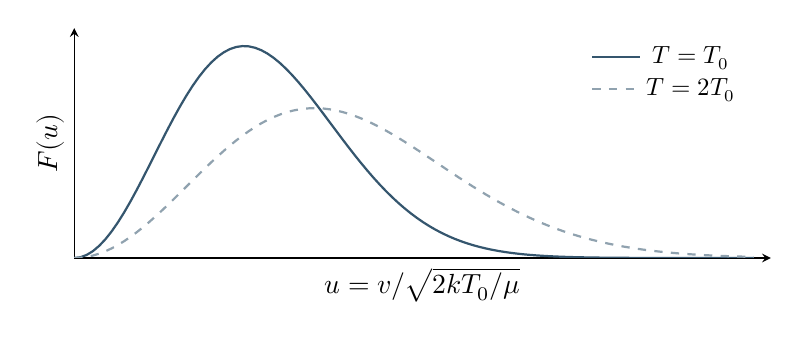
\begin{tikzpicture}
\begin{axis}[width=.86\linewidth,height=4.5cm,axis lines=left,
 xlabel={$u=v/\sqrt{2kT_0/\mu}$},ylabel={$F(u)$},
 xmin=0,xmax=4.1,ymin=0,ymax=.9,domain=0:4,samples=110,
 ticks=none,legend style={draw=none,font=\small,at={(.97,.97)},anchor=north east}]
\addplot[ThemeMain,thick]{4/sqrt(pi)*x^2*exp(-x^2)};
\addlegendentry{$T=T_0$}
\addplot[ThemeMain!55!white,thick,dashed]{4/sqrt(pi)/2^1.5*x^2*exp(-x^2/2)};
\addlegendentry{$T=2T_0$}
\end{axis}
\end{tikzpicture}
\par\small 同一种气体的无量纲速率分布。$T_0$ 为参考温度，$F(u)\dd u=f(v)\dd v$。
\end{center}

\subsection{三种统计速率及其推导}
\term{最概然速率} $v_{\mathrm p}$ 对应分布密度的最大值。对 $v>0$ 令 $\dd(\ln f)/\dd v=0$：
\[
 \frac{2}{v}-\frac{\mu v}{kT}=0
 \quad\Longrightarrow\quad v_{\mathrm p}=\sqrt{\frac{2kT}{\mu}}.
\]
\term{平均速率}与\term{方均根速率}分别定义为
\[
 \bar v=\int_0^\infty vf(v)\dd v,
 \qquad v_{\mathrm{rms}}=\sqrt{\int_0^\infty v^2f(v)\dd v}.
\]
令 $a=\mu/(2kT)>0$。利用
\[
 \int_0^\infty v^3\ee^{-av^2}\dd v=\frac{1}{2a^2},
 \qquad
 \int_0^\infty v^4\ee^{-av^2}\dd v=\frac{3\sqrt\pi}{8a^{5/2}},
\]
代入 $f(v)$ 得
\begin{infobox}[breakable=false]{结论：三种统计速率}
\[
 v_{\mathrm p}=\sqrt{\frac{2RT}{M}},\qquad
 \bar v=\sqrt{\frac{8RT}{\pi M}},\qquad
 v_{\mathrm{rms}}=\sqrt{\overline{v^2}}=\sqrt{\frac{3RT}{M}}.
\]
对麦克斯韦分布，$v_{\mathrm p}<\bar v<v_{\mathrm{rms}}$。平均平动动能使用 $\overline{v^2}$，不能替换为 $\bar v^{\,2}$。
\end{infobox}
例如，$300\unit K$ 的氮气，取 $M=28.0\times10^{-3}\unit{kg\,mol^{-1}}$，有 $v_{\mathrm p}\approx422\unit{m\,s^{-1}}$、$\bar v\approx476\unit{m\,s^{-1}}$、$v_{\mathrm{rms}}\approx517\unit{m\,s^{-1}}$。这些是同一分布的不同统计量，不能理解成每个分子只具有三种可能速率。

\subsection{给定分布的归一化与平均值}
\begin{infobox}{例题：三角形速率分布}
总分子数为 $N$，分子数密度曲线 $Nf(v)$ 在 $v=0$ 和 $v=3v_0$ 处为零，在 $v=v_0$ 处达到峰值 $a$，两段均为直线，其中 $v_0>0$。求 $a$、最概然速率和平均速率。
\end{infobox}
\sol 曲线下面积为 $N$，所以
\[
 \frac12(3v_0)a=N,\qquad a=\frac{2N}{3v_0}.
\]
分布可明确写成
\[
 Nf(v)=\begin{cases}
 av/v_0,&0\le v\le v_0,\\
 a(3v_0-v)/(2v_0),&v_0<v\le3v_0,\\
 0,&\text{其他速率}.
 \end{cases}
\]
峰值位置给出 $v_{\mathrm p}=v_0$。平均速率须对整个曲线积分：
\begin{align*}
 \bar v&=\frac aN\left[
 \int_0^{v_0}\frac{v^2}{v_0}\dd v+
 \int_{v_0}^{3v_0}\frac{v(3v_0-v)}{2v_0}\dd v\right]\\
 &=\frac aN\left(\frac{v_0^2}{3}+\frac{5v_0^2}{3}\right)
 =\frac43v_0.
\end{align*}
若只求 $[0,v_0]$ 内分子的平均速率，则
\[
 \bar v_{[0,v_0]}=
 \frac{av_0^2/3}{av_0/2}=\frac23v_0.
\]
分布不是麦克斯韦分布时，不能直接套用理想气体的三种速率公式。

\begin{infobox}{例题：具有速率上限的给定分布}
给定 $f(v)=Av^2$（$0\le v\le v_{\mathrm F}$），在此区间外为零，$v_{\mathrm F}>0$ 为速率上限。求归一化常数、平均速率和方均根速率。
\end{infobox}
\sol 由 $Av_{\mathrm F}^3/3=1$，得 $A=3/v_{\mathrm F}^3$。于是
\[
 \bar v=\frac{3}{v_{\mathrm F}^3}\int_0^{v_{\mathrm F}}v^3\dd v
 =\frac34v_{\mathrm F},\qquad
 v_{\mathrm{rms}}=\sqrt{\frac35}\,v_{\mathrm F}.
\]
密度在上边界最大，通常记最概然速率为 $v_{\mathrm F}$。这类截断分布可作为电子气的给定模型练习，但不能据此把金属中的简并电子当作服从经典麦克斯韦分布的气体。

\subsection{速率分布实验的基本原理}
分子束通过两处狭缝的距离为 $\ell$，飞行时间为 $\tau=\ell/v$。若装置以角速度 $\omega$ 转动，在飞行期间转过的角度为 $\theta=\omega\tau$，则
\[
 v=\frac{\omega\ell}{\theta},
\]
其中 $\theta$ 用弧度表示。由偏转或位移与速率的对应关系，可测定分子束的速率分布。实验束流会对快分子加权，直接测得的束流分布与容器中分子数的速率分布须按实验取样方式区分。

\subsection{玻耳兹曼分布与重力场中的气体}
\term{玻耳兹曼分布}（Boltzmann distribution）描述经典热平衡中微观状态的能量权重。能量为 $\varepsilon$ 的单个微观状态，其概率正比于 $\ee^{-\varepsilon/(kT)}$。对能量区间内的分子数，还要计入该区间包含的状态数，不能仅凭指数因子断言能量分布密度单调下降。

设保守力场中单分子势能为 $\varepsilon_{\mathrm p}(\symbf r)$，$\symbf r=(x,y,z)$，且系统温度处处为 $T$。平动能与势能可分离，六维空间中的分子数分布为
\begin{align*}
 \dd N={}&n_0\left(\frac{\mu}{2\pi kT}\right)^{3/2}
 \exp\left[-\frac{\varepsilon_{\mathrm{kt}}+
 \varepsilon_{\mathrm p}(\symbf r)}{kT}\right]\\
 &\hspace{1em}\cdot\dd x\dd y\dd z\dd v_x\dd v_y\dd v_z.
\end{align*}
$n_0$ 为势能取零处的数密度。对三个速度分量积分，利用麦克斯韦速度分布的归一化，有
\[
 n(\symbf r)=n_0\ee^{-\varepsilon_{\mathrm p}(\symbf r)/(kT)}.
\]
位置改变影响数密度；在给定位置按当地分子数重新归一化后，速率分布仍是相同温度 $T$ 下的麦克斯韦分布。这是群体平衡的结论，并不否定单个上升分子动能转化为势能。

\begin{infobox}{核心公式：等温气压公式}
取竖直向上坐标 $z$，令 $z=0$ 处势能为零。对单一理想气体，在温度 $T$、重力加速度 $g$ 均为常量的近似下，
\[
 n(z)=n_0\ee^{-\mu gz/(kT)},\qquad
 p(z)=p_0\ee^{-Mgz/(RT)}.
\]
$p_0$ 为 $z=0$ 处压强。特征高度 $H=RT/(Mg)$，在 $z=H$ 处压强降至 $p_0/\ee$。
\end{infobox}
该式也可由静力平衡推导：厚度为 $\dd z$、横截面积为 $A$ 的气层满足
\[
 A[p(z)-p(z+\dd z)]=\rho gA\dd z,
\]
从而 $\dd p/\dd z=-\rho g$。代入 $\rho=pM/(RT)$ 并积分，即得等温气压公式。真实大气的温度、组成及 $g$ 可随高度改变，不能在任意高度范围直接采用一个恒定的气压下降率。


\chapterpage{真实气体、碰撞与平均自由程}
\subsection{真实气体等温线与临界状态}
\term{真实气体}的分子具有有限大小及相互作用。对纯物质，当温度低于\term{临界温度} $T_{\mathrm c}$ 时，缓慢等温压缩可能经过气体、汽液共存和液体三个区域。在汽液共存阶段，继续压缩主要使蒸气液化，平衡压强保持在该温度的\term{饱和蒸气压}。

随温度升高，汽液共存的体积区间缩短；到临界点，气相与液相的差别消失。$T>T_{\mathrm c}$ 时，单凭等温加压不能得到具有汽液相界面的液化过程。低于临界温度也不意味着任意压强下气体都会液化。

\subsection{范德瓦耳斯方程及两项修正}
\term{范德瓦耳斯方程}（van der Waals equation）对理想气体方程加入排除体积和分子吸引的近似修正。对 $\nu$ 摩尔气体，
\begin{infobox}{模型：范德瓦耳斯状态方程}
\[
 \left(p+\frac{a\nu^2}{V^2}\right)(V-\nu b)=\nu RT.
\]
$a>0$ 为吸引作用参数，单位 $\mathrm{Pa\,m^6\,mol^{-2}}$；$b>0$ 为排除体积参数，单位 $\mathrm{m^3\,mol^{-1}}$。模型要求 $V>\nu b$。
\end{infobox}
可供分子运动的有效体积近似取 $V-\nu b$。$b$ 是每摩尔的排除体积参数，不等同于分子实体积的简单总和。分子间吸引使实际器壁压强比不计吸引时小，需补加 $a\nu^2/V^2$ 后再与理想动理模型的压强对应。

令摩尔体积 $V_{\mathrm m}=V/\nu$，可写成
\[
 p=\frac{RT}{V_{\mathrm m}-b}-\frac{a}{V_{\mathrm m}^2}.
\]
当 $V_{\mathrm m}\gg b$ 且 $a/V_{\mathrm m}^2\ll p$ 时，退化为理想气体近似。模型临界点满足
\[
 \left(\frac{\partial p}{\partial V_{\mathrm m}}\right)_T=0,
 \qquad
 \left(\frac{\partial^2p}{\partial V_{\mathrm m}^2}\right)_T=0.
\]
对上述方程求导，得到
\[
 -\frac{RT}{(V_{\mathrm m}-b)^2}+\frac{2a}{V_{\mathrm m}^3}=0,
 \qquad
 \frac{2RT}{(V_{\mathrm m}-b)^3}-\frac{6a}{V_{\mathrm m}^4}=0.
\]
消去 $T$，有 $V_{\mathrm m,c}=3b$，再代回得到
\[
 T_{\mathrm c}=\frac{8a}{27Rb},\qquad
 p_{\mathrm c}=\frac{a}{27b^2}.
\]
范德瓦耳斯等温线在亚临界区的回折段不能直接视作稳定的平衡过程。真实平衡的汽液共存由水平共存段描述；该模型是定性及近似定量模型，尤其在临界区并非精确状态方程。

\subsection{平均碰撞频率与平均自由程}
采用相同分子、直径为 $d$ 的无引力硬球模型，有效碰撞截面为 $\sigma=\pi d^2$。这里 $d$ 是碰撞直径，而 $\sigma$ 是面积，二者不能混用。

若其他分子暂时静止，单个分子以速率 $u$ 运动，在时间 $\dd t$ 内扫过体积 $\pi d^2u\dd t$，预计碰撞数为 $n\pi d^2u\dd t$。真实气体中双方都运动，应将 $u$ 换成相对速率的平均。对同种、同温的麦克斯韦分布，$\overline{v_{\mathrm{rel}}}=\sqrt2\bar v$，于是
\begin{infobox}{核心公式：硬球模型的碰撞统计}
\[
 \bar z=\sqrt2\pi d^2n\bar v,
 \qquad
 \lambda=\frac{\bar v}{\bar z}
 =\frac{1}{\sqrt2\pi d^2n}
 =\frac{kT}{\sqrt2\pi d^2p}.
\]
$\bar z$ 是每个分子单位时间内的平均碰撞次数，单位 $\mathrm{s^{-1}}$；$\lambda$ 是相邻两次分子间碰撞之间路程的平均值，单位 $\mathrm m$。
\end{infobox}
总分子间碰撞次数率为 $N\bar z/2$，因一次碰撞涉及两个分子。总碰撞次数率与单分子碰撞频率不能混为一谈。

固定气体种类并近似认为 $d$ 不变时，$\bar v\propto\sqrt T$，因而
\begin{center}
\begin{tabularx}{\linewidth}{l Y Y}
\toprule
改变条件 & 平均自由程 $\lambda$ & 平均碰撞频率 $\bar z$\\
\midrule
定温增压 & $\lambda\propto p^{-1}$，减小 & $\bar z\propto p$，增大\\
定压升温 & $\lambda\propto T$，增大 & $\bar z\propto T^{-1/2}$，减小\\
定容、定分子数升温 & $n$ 不变，$\lambda$ 不变 & $\bar z\propto T^{1/2}$，增大\\
固定 $n,T$，增大 $d$ & $\lambda\propto d^{-2}$，减小 & $\bar z\propto d^2$，增大\\
\bottomrule
\end{tabularx}
\end{center}
定压升温时，速率虽增大，但数密度 $n=p/(kT)$ 降低，后一效应占优势。因此不能仅凭分子运动变快判断碰撞频率增大。

\begin{infobox}{例题：标准状态下氢气的碰撞统计}
取 $T=273.15\unit K$、$p=1.01325\times10^5\unit{Pa}$、$M=2.00\times10^{-3}\unit{kg\,mol^{-1}}$、$d=2.00\times10^{-10}\unit m$，求氢气的 $\bar v,n,\lambda,\bar z$。
\end{infobox}
\sol 依次由速率公式、状态方程及碰撞公式计算：
\begin{align*}
 \bar v&=\sqrt{\frac{8RT}{\pi M}}\approx1.70\times10^3\unit{m\,s^{-1}},\\
 n&=\frac p{kT}\approx2.69\times10^{25}\unit{m^{-3}},\\
 \lambda&=\frac1{\sqrt2\pi d^2n}\approx2.09\times10^{-7}\unit m,\\
 \bar z&=\frac{\bar v}{\lambda}\approx8.13\times10^9\unit{s^{-1}}.
\end{align*}
结果表明分子运动速率很大，碰撞也极频繁；宏观扩散速度不能直接等同于单分子的平均速率。

\subsection{稀薄气体与真空技术的物理基础}
压强很低时，分子间平均自由程可能超过容器特征长度 $L$。此时分子与器壁的碰撞对输运更重要，但分子间平均自由程公式的含义没有变，不能直接把计算得到的 $\lambda$ 改写成 $L$。若讨论分子在容器内的有效直线路程，则必须另外考虑几何边界。

\term{克努森数} $\mathrm{Kn}=\lambda/L$ 比较自由程与装置尺度。$\mathrm{Kn}$ 很小时适合连续介质近似；$\mathrm{Kn}$ 较大时需考虑稀薄气体效应。真空程度用绝对压强表示，压强越小，通常所谓“真空度”越高；$1\unit{Torr}=(101325/760)\unit{Pa}\approx133.322\unit{Pa}$。

对均匀气体，在近似恒定碰撞率下，路程 $\ell$ 内不发生碰撞的概率为
\[
 P_0(\ell)=\ee^{-\ell/\lambda}.
\]
走过一个平均自由程时，仍约有 $\ee^{-1}\approx36.8\%$ 的分子未碰撞。平均自由程不是每个分子的固定路程。

在热平衡且器壁静止时，单位面积、单位时间的入射分子数称为\term{入射通量} $J$。由正向法向速度平均得
\[
 J=n\int_0^\infty v_x\phi(v_x)\dd v_x
 =\frac14n\bar v
 =\frac{p}{\sqrt{2\pi\mu kT}}.
\]
$J$ 的单位为 $\mathrm{m^{-2}\,s^{-1}}$，与单位为 $\mathrm{s^{-1}}$ 的 $\bar z$ 不同。若表面单分子层的容纳密度为 $n_{\mathrm s}$、吸附概率近似为 1，覆盖时间约为 $n_{\mathrm s}/J$；降低压强可延长表面的洁净保持时间。真空蒸发镀膜还要求蒸发粒子的相关碰撞自由程远大于源与基片的距离，以减少飞行途中散射。空间环境模拟的低压条件同样与稀薄气体效应有关；真空本身不等同于失重。

\chapterpage{热力学第一定律与热容}
\subsection{功、热量与内能的区别}
\term{功} $W$ 和\term{热量} $Q$ 描述能量传递的方式。热量由温差引起的能量交换产生；功由宏观有序作用引起。系统“具有”内能，不能说系统“具有某一热量”。内能是\term{状态量}，而功和热量是\term{过程量}。

\begin{infobox}{约定：热量和功的正负}
$Q>0$ 表示系统吸热，$Q<0$ 表示系统放热；$W>0$ 表示系统对外做功，$W<0$ 表示外界对系统做功。固定组成的封闭系统，且忽略整体机械能变化时，\term{热力学第一定律}为
\[
 Q=\Delta E+W,\qquad \dd E=\delta Q-\delta W.
\]
$\delta Q,\delta W$ 表示微小过程中的能量传递，$\dd E$ 表示状态函数的全微分。
\end{infobox}
若系统整体动能或外场势能改变，应把它们一并计入能量守恒；若还有电功等其他功形式，也须计入 $W$。第一定律本身不要求过程准静态或可逆。

状态量满足 $\Delta E=E_2-E_1$，循环后 $\Delta E=0$；两个相同端点之间，$Q$ 和 $W$ 可因路径不同而不同，但 $Q-W$ 始终相同。

若一台循环装置不从外界获得能量，却持续对外做功，就违背能量守恒；这种装置称为\term{第一类永动机}，不能实现。

\subsection{体积功及其适用条件}
设活塞面积为 $A$，向外位移为 $\dd x$，则体积变化 $\dd V=A\dd x$。外界阻力对应的外压为 $p_{\mathrm{ext}}$，边界功为
\[
 \delta W=p_{\mathrm{ext}}\dd V,
 \qquad W=\int_{V_1}^{V_2}p_{\mathrm{ext}}\dd V.
\]
对无摩擦、机械准静态的极限过程，内压与外压只相差无穷小量，可采用系统平衡压强 $p$：
\[
 W=\int_{V_1}^{V_2}p\dd V.
\]
膨胀时 $\dd V>0$，气体对外做正功；压缩时做负功。在 $p$--$V$ 图中，该积分为过程曲线下的有向面积。非准静态自由膨胀的系统压强无法沿过程均匀定义，也不能把初末态之间的等温线面积当成实际功。

\subsection{热容量、比热容和摩尔热容}
\term{热容量}取决于系统及过程。在可用温度变化表征的指定过程 $\mathcal P$ 上，
\[
 C_{\mathcal P}=\frac{\delta Q}{\dd T},\qquad
 c_{\mathcal P}=\frac1m\frac{\delta Q}{\dd T},\qquad
 C_{\mathcal P,\mathrm m}=\frac1\nu\frac{\delta Q}{\dd T}.
\]
$c_{\mathcal P}$ 为\term{比热容}，$C_{\mathcal P,\mathrm m}$ 为\term{摩尔热容}，单位依次为 $\mathrm{J\,K^{-1}}$、$\mathrm{J\,kg^{-1}\,K^{-1}}$、$\mathrm{J\,mol^{-1}\,K^{-1}}$。等温过程有 $\dd T=0$，不能用一个有限的过程热容描述。

对于只做体积功的气体，\term{定容摩尔热容}与\term{定压摩尔热容}分别为
\[
 C_{V,\mathrm m}=\frac1\nu\left(\frac{\delta Q}{\dd T}\right)_V,
 \qquad
 C_{p,\mathrm m}=\frac1\nu\left(\frac{\delta Q}{\dd T}\right)_p.
\]
理想气体的 $E$ 只依赖 $T$，由定容过程 $\delta Q=\dd E$ 得
\[
 \dd E=\nu C_{V,\mathrm m}(T)\dd T,
 \qquad \Delta E=\nu\int_{T_1}^{T_2}C_{V,\mathrm m}(T)\dd T.
\]
该内能变化公式对连接相同平衡端点的任意过程都成立，因为它表达状态函数变化；不能据此把任意过程的实际吸热也写成同一积分。

\subsection{迈耶公式与热容比}
定压、机械准静态过程中，$\delta Q=\dd E+p\dd V$。由 $pV=\nu RT$，在 $p$ 固定时 $p\dd V=\nu R\dd T$，所以
\[
 \nu C_{p,\mathrm m}\dd T
 =\nu C_{V,\mathrm m}\dd T+\nu R\dd T.
\]
\begin{infobox}{结论：理想气体热容关系}
\[
 C_{p,\mathrm m}-C_{V,\mathrm m}=R,
 \qquad \gamma=\frac{C_{p,\mathrm m}}{C_{V,\mathrm m}}.
\]
$\gamma$ 为\term{热容比}。若有效能量自由度 $i$ 不变，
\[
 C_{V,\mathrm m}=\frac i2R,\quad
 C_{p,\mathrm m}=\frac{i+2}{2}R,\quad
 \gamma=\frac{i+2}{i}.
\]
\end{infobox}
单原子、刚性线性分子、刚性非线性分子模型分别给出 $\gamma=5/3,7/5,4/3$。迈耶公式在固定组成的理想气体中成立，即使热容随温度变化，仍可逐温度使用；常数热容公式则需要额外检验温度范围。

\chapterpage{理想气体的典型过程}
本章除自由膨胀外，均讨论物质的量 $\nu$ 不变、只做体积功的机械准静态过程。涉及显式常数公式时，假定 $C_{V,\mathrm m}$、$C_{p,\mathrm m}$ 以及 $\gamma$ 不随温度变化。记 $\Delta T=T_2-T_1$。

\subsection{等容、等压与等温过程}
\term{等容过程}满足 $V$ 不变，因此 $W=0$，$p/T$ 不变。由第一定律，
\[
 Q_V=\Delta E=\nu C_{V,\mathrm m}\Delta T.
\]
等容升温时，吸收的热量全部用于增加内能。

\term{等压过程}满足 $p$ 不变，因此 $V/T$ 不变。功、内能变化和热量为
\begin{align*}
 W&=p(V_2-V_1)=\nu R\Delta T,\\
 \Delta E&=\nu C_{V,\mathrm m}\Delta T,\\
 Q_p&=\nu C_{p,\mathrm m}\Delta T.
\end{align*}
等压升温还需对外做功，同样的温升所需热量比等容过程大。

\term{等温过程}满足 $T$ 不变。对理想气体，$\Delta E=0$，$p=\nu RT/V$，因此
\begin{align*}
 W&=\int_{V_1}^{V_2}\frac{\nu RT}{V}\dd V
 =\nu RT\ln\frac{V_2}{V_1},\\
 Q_T&=W=\nu RT\ln\frac{p_1}{p_2}.
\end{align*}
等温膨胀过程中虽温度不升高，仍须吸热补偿对外做功所消耗的能量。$\Delta E=0$ 依赖理想气体内能只随温度变化的性质，不能直接推广到任意真实物质。

\begin{infobox}{例题：相同热量对应的三种过程}
将 $Q=500\unit J$ 分别传给初态相同的 $2.00\unit{mol}$ 氢气。初温 $T_0=273.15\unit K$，初压 $p_0=1.01325\times10^5\unit{Pa}$。采用 $i=5$ 的理想气体模型，分别求等容、等温及等压吸热后的状态。
\end{infobox}
\sol 初体积 $V_0=\nu RT_0/p_0\approx4.483\times10^{-2}\unit{m^3}$。
\begin{enumerate}
\item 等容：$W=0$、$\Delta E=500\unit J$，
\[
 T=T_0+\frac{Q}{\nu(5R/2)}\approx285.18\unit K,
 \qquad p=p_0\frac{T}{T_0}\approx1.058\times10^5\unit{Pa}.
\]
\item 等温：$\Delta E=0$、$W=500\unit J$，
\[
 V=V_0\exp\left(\frac{Q}{\nu RT_0}\right)
 \approx5.004\times10^{-2}\unit{m^3},
 \qquad p\approx9.076\times10^4\unit{Pa}.
\]
\item 等压：
\[
 T=T_0+\frac{Q}{\nu(7R/2)}\approx281.74\unit K,
 \qquad V=V_0\frac{T}{T_0}\approx4.624\times10^{-2}\unit{m^3}.
\]
$\Delta E=(5/7)Q\approx357.14\unit J$，$W=(2/7)Q\approx142.86\unit J$。
\end{enumerate}
三种情况下吸热相同，但功、内能变化和末态不同，说明热量属于过程量。

\subsection{可逆绝热过程及绝热方程}
\term{绝热过程}满足 $\delta Q=0$。若过程还可逆且只做体积功，则
\[
 \nu C_{V,\mathrm m}\dd T=-p\dd V.
\]
代入 $p=\nu RT/V$，约去 $\nu$，有
\[
 \frac{\dd T}{T}+\frac{R}{C_{V,\mathrm m}}\frac{\dd V}{V}=0.
\]
由 $R/C_{V,\mathrm m}=\gamma-1$ 并在常数热容条件下积分，
\[
 \ln T+(\gamma-1)\ln V=\text{常量}.
\]
再利用状态方程消去 $T$ 或 $V$，得到
\begin{infobox}{核心公式：可逆绝热方程}
\[
 TV^{\gamma-1}=\text{常量},\qquad
 pV^\gamma=\text{常量},\qquad
 T^\gamma p^{1-\gamma}=\text{常量}.
\]
这些方程要求固定组成的理想气体、常数热容以及可逆绝热过程；仅有 $Q=0$ 并不足以使用。
\end{infobox}
绝热功由能量守恒得到
\[
 W=-\Delta E=\nu C_{V,\mathrm m}(T_1-T_2)
 =\frac{p_1V_1-p_2V_2}{\gamma-1}.
\]
在同一状态 $(p,V)$，等温线和可逆绝热线的斜率分别为
\[
 \left(\frac{\dd p}{\dd V}\right)_T=-\frac pV,
 \qquad
 \left(\frac{\dd p}{\dd V}\right)_{\mathrm{ad}}=-\gamma\frac pV.
\]
因 $\gamma>1$，绝热线斜率的绝对值较大，其代数值更小。说“斜率较大”时必须指明比较的是绝对值。

\begin{center}
\begin{tikzpicture}
\begin{axis}[width=.78\linewidth,height=4.8cm,axis lines=left,
 xlabel={$V/V_1$},ylabel={$p/p_1$},xmin=.9,xmax=3.2,ymin=0,ymax=1.2,
 domain=1:3,samples=80,legend style={draw=none,font=\small}]
\addplot[ThemeMain,thick]{1/x};\addlegendentry{等温}
\addplot[ThemeMain!60!white,thick,dashed]{x^(-1.4)};\addlegendentry{可逆绝热}
\end{axis}
\end{tikzpicture}
\par\small 从同一初态膨胀时，$\gamma=1.4$ 的可逆绝热线下降较快。
\end{center}

\subsection{绝热自由膨胀}
气体在隔热刚性容器内向真空区域扩展称为\term{绝热自由膨胀}。容器与外界无热量交换，气体向真空扩展不克服外压，所以
\[
 Q=0,\quad W=0,\quad\Delta E=0.
\]
若固定组成的理想气体由初平衡态最终达到另一个平衡态，因 $E=E(T)$，有 $T_2=T_1$；又因 $V_2>V_1$，有 $p_2<p_1$。过程的中间状态并非平衡态，不能套用 $pV^\gamma=\text{常量}$。真实气体即使 $\Delta E=0$，温度也可能改变。

\subsection{多方过程及过程热容}
\term{多方过程}是满足 $pV^q=K_q$ 的机械准静态过程，其中 $q$ 为固定的多方指数，$K_q$ 为该过程的常量。它可用于近似描述多种实际过程，并不限于介于等温与绝热之间的情形。

当 $q\ne1$ 时，
\begin{align*}
 W&=K_q\int_{V_1}^{V_2}V^{-q}\dd V
 =\frac{p_2V_2-p_1V_1}{1-q}\\
 &=\frac{\nu R(T_2-T_1)}{1-q},\\
 Q&=\Delta E+W
 =\nu\left(C_{V,\mathrm m}+\frac{R}{1-q}\right)\Delta T.
\end{align*}
相应的过程摩尔热容为
\[
 C_{q,\mathrm m}=C_{V,\mathrm m}+\frac R{1-q}
 =C_{V,\mathrm m}\frac{\gamma-q}{1-q}.
\]
$q=0$ 对应等压，$q=1$ 对应等温，$q=\gamma$ 对应满足前述条件的可逆绝热。等容过程通常作为 $q\to\infty$ 的极限理解，不能把“无穷大”当作普通有限指数直接代入计算。

在 $1<q<\gamma$ 的膨胀中，$T$ 降低而 $Q>0$，所以 $C_{q,\mathrm m}<0$。这不违背能量守恒：吸热小于对外做功，差额来自内能减少。过程热容为负不表示定容热容为负。

\subsection{过程公式比较与计算步骤}
下表仅在本章说明的固定物质的量、理想气体及常数热容条件下使用。表中 $W$ 均采用系统对外做功为正的约定。
\begin{center}
\small
\begin{tabularx}{\linewidth}{l Y Y Y}
\toprule
过程 & 状态约束 & 对外功 $W$ & 吸热 $Q$\\
\midrule
等容 & $V=\text{常量}$ & $0$ & $\nu C_{V,\mathrm m}\Delta T$\\
等压 & $p=\text{常量}$ & $\nu R\Delta T$ & $\nu C_{p,\mathrm m}\Delta T$\\
等温 & $T=\text{常量}$ & $\nu RT\ln(V_2/V_1)$ & $W$\\
可逆绝热 & $pV^\gamma=\text{常量}$ & $-\nu C_{V,\mathrm m}\Delta T$ & $0$\\
多方，$q\ne1$ & $pV^q=\text{常量}$ & $\nu R\Delta T/(1-q)$ & $\nu C_{q,\mathrm m}\Delta T$\\
\bottomrule
\end{tabularx}
\end{center}
所有过程的内能变化均为 $\Delta E=\nu C_{V,\mathrm m}\Delta T$。实际过程只要初末态确定，即可先求 $\Delta E$，但求 $W,Q$ 必须知道路径及相应条件。

\begin{infobox}{方法：多阶段气体过程}
先确认系统、符号约定及模型；将摄氏温度和摩尔质量换为国际单位；根据每段状态约束逐一求端点；分别计算各段 $\Delta E,W,Q$；最后求和，并以总关系 $Q_{\mathrm{tot}}-W_{\mathrm{tot}}=E_{\mathrm{final}}-E_{\mathrm{initial}}$ 核对。
\end{infobox}

\begin{infobox}{例题：等容、等温、等压组成的过程}
$0.100\unit{mol}$ 氮气由 A 态 $T_A=300\unit K$、$p_A=p_0$ 出发，先等容使压强变为 $3p_0$（B 态），再等温膨胀到 $p_0$（C 态），最后等压压缩至 C 态体积的一半（D 态）。取 $i=5$，求整个过程的 $\Delta E,W,Q$。
\end{infobox}
\sol 由各段状态约束，
\[
 T_B=T_C=900\unit K,\quad V_B=V_A,\quad
 V_C=3V_A,\quad V_D=\frac32V_A,\quad T_D=450\unit K.
\]
逐段计算如下（数值单位为焦耳）：
\begin{center}
\begin{tabular}{l r r r}
\toprule
过程 & $\Delta E$ & $W$ & $Q$\\
\midrule
A$\to$B & $1247.2$ & $0$ & $1247.2$\\
B$\to$C & $0$ & $822.1$ & $822.1$\\
C$\to$D & $-935.4$ & $-374.2$ & $-1309.5$\\
\midrule
总计 & $311.8$ & $447.9$ & $759.7$\\
\bottomrule
\end{tabular}
\end{center}
其中等温段 $W_{BC}=0.100R\times900\ln3$。总内能变化也可直接由初末温度得到 $\Delta E=0.100(5R/2)(450-300)$，与逐段和一致。

\chapterpage{循环过程、热机与制冷机}
\subsection{循环过程与有向面积}
\term{循环过程}是系统经历若干状态变化后回到初态的过程。任何状态函数在一个完整循环后的增量为零，因此
\[
 \Delta E_{\mathrm{cyc}}=0,\qquad W_{\mathrm{cyc}}=Q_{\mathrm{net}}.
\]
机械准静态循环的净功为
\[
 W_{\mathrm{cyc}}=\oint p\dd V.
\]
通常的单个封闭回路在 $p$--$V$ 图上顺时针运行时净功为正，逆时针时为负，大小为所围面积。复杂回路须按有向面积相加，不能只看总几何面积。

\subsection{热机效率与制冷系数}
\term{热机}从高温热源吸热并输出净功，同时向低温热源放热。定义 $Q_{\mathrm H}>0$ 为从高温热源吸收的热量，$Q_{\mathrm L}>0$ 为向低温热源放出的热量大小，则
\[
 W_{\mathrm{out}}=Q_{\mathrm H}-Q_{\mathrm L},\qquad
 \eta=\frac{W_{\mathrm{out}}}{Q_{\mathrm H}}
 =1-\frac{Q_{\mathrm L}}{Q_{\mathrm H}}.
\]
这里 $Q_{\mathrm L}$ 是正的大小；若仍用有符号的低温段热量，应写 $Q_{\mathrm{cold}}=-Q_{\mathrm L}$。

\term{制冷机}消耗外界输入功 $W_{\mathrm{in}}>0$，从低温处吸取 $Q_{\mathrm L}>0$，并向高温处放出 $Q_{\mathrm H}>0$：
\[
 W_{\mathrm{in}}=Q_{\mathrm H}-Q_{\mathrm L},\qquad
 \varepsilon=\frac{Q_{\mathrm L}}{W_{\mathrm{in}}}
 =\frac{Q_{\mathrm L}}{Q_{\mathrm H}-Q_{\mathrm L}}.
\]
$\varepsilon$ 为\term{制冷系数}，也称性能系数（COP），可以大于 1，因为分子是搬运的热量，并非由功全部转化产生的能量。

\subsection{卡诺循环及效率推导}
\term{卡诺循环}由两个可逆等温过程和两个可逆绝热过程组成，只与温度恒定的两个热源交换热量。设高温 $T_{\mathrm H}$、低温 $T_{\mathrm L}$ 满足 $T_{\mathrm H}>T_{\mathrm L}>0$。理想气体正向循环的四段为
\begin{enumerate}
\item A$\to$B：在 $T_{\mathrm H}$ 下可逆等温膨胀，吸热；
\item B$\to$C：可逆绝热膨胀，温度降到 $T_{\mathrm L}$；
\item C$\to$D：在 $T_{\mathrm L}$ 下可逆等温压缩，放热；
\item D$\to$A：可逆绝热压缩，温度升到 $T_{\mathrm H}$。
\end{enumerate}
\begin{center}
\begin{minipage}{\linewidth}
\centering
\begin{tikzpicture}
\begin{axis}[width=.82\linewidth,height=5.0cm,axis lines=left,
 xlabel={$V/V_A$},ylabel={$p/p_A$},xmin=.75,xmax=3.5,ymin=.12,ymax=1.18,
 ticks=none,clip=false]
\addplot[ThemeMain,thick,domain=1:1.8,samples=60]{1/x};
\addplot[ThemeMain,thick,dashed,domain=1.8:3.14447,samples=60]{1.8^(.4)*x^(-1.4)};
\addplot[ThemeMain,thick,domain=1.74693:3.14447,samples=60]{.8/x};
\addplot[ThemeMain,thick,dashed,domain=1:1.74693,samples=60]{x^(-1.4)};
\node[above left] at (axis cs:1,1) {A};
\node[above right] at (axis cs:1.8,.55556) {B};
\node[below right] at (axis cs:3.14447,.254415) {C};
\node[below left] at (axis cs:1.74693,.457947) {D};
\draw[ThemeMain,-{Stealth[length=2mm]}] (axis cs:1.35,.74074)--(axis cs:1.46,.68493);
\draw[ThemeMain,-{Stealth[length=2mm]}] (axis cs:2.3,.39414)--(axis cs:2.45,.36078);
\draw[ThemeMain,-{Stealth[length=2mm]}] (axis cs:2.6,.30769)--(axis cs:2.45,.32653);
\draw[ThemeMain,-{Stealth[length=2mm]}] (axis cs:1.45,.59457)--(axis cs:1.35,.65688);
\end{axis}
\end{tikzpicture}
\par\small 理想气体卡诺循环示意：实线为等温段，虚线为绝热段，箭头表示正向循环。
\end{minipage}
\end{center}

对常数热容理想气体，两条绝热线分别给出
\[
 T_{\mathrm H}V_B^{\gamma-1}=T_{\mathrm L}V_C^{\gamma-1},\qquad
 T_{\mathrm H}V_A^{\gamma-1}=T_{\mathrm L}V_D^{\gamma-1}.
\]
相除得 $V_B/V_A=V_C/V_D$。两个等温过程的热量大小为
\[
 Q_{\mathrm H}=\nu RT_{\mathrm H}\ln\frac{V_B}{V_A},\qquad
 Q_{\mathrm L}=\nu RT_{\mathrm L}\ln\frac{V_C}{V_D}.
\]
因此 $Q_{\mathrm L}/Q_{\mathrm H}=T_{\mathrm L}/T_{\mathrm H}$，得到
\begin{infobox}{核心公式：卡诺效率与卡诺制冷系数}
\[
 \eta_{\mathrm C}=1-\frac{T_{\mathrm L}}{T_{\mathrm H}},
 \qquad
 \varepsilon_{\mathrm C}=\frac{T_{\mathrm L}}{T_{\mathrm H}-T_{\mathrm L}}.
\]
温度必须使用开尔文。卡诺循环可逆，式中温度为两个恒温热源的温度，不能把任意循环的最高、最低气体温度直接代入。
\end{infobox}
若 $T_{\mathrm H}=580\,{}^\circ\mathrm C$、$T_{\mathrm L}=30\,{}^\circ\mathrm C$，则 $\eta_{\mathrm C}=1-303.15/853.15\approx64.5\%$。这是两热源间的可逆上限，不能直接当作实际电厂效率。

\begin{infobox}{例题：固定两条绝热线时的循环净功}
一卡诺热机的初始高温热源为 $100\,{}^\circ\mathrm C$，低温热源为 $0\,{}^\circ\mathrm C$。保持低温热源及两条绝热线不变，若每循环净功加倍，求新的高温热源温度和效率。
\end{infobox}
\sol 固定两条绝热线使两个等温段的体积比不变，记 $r=V_B/V_A=V_C/V_D$。于是
\[
 W=\nu R(T_{\mathrm H}-T_{\mathrm L})\ln r.
\]
由 $W'=2W$，
\[
 T_{\mathrm H}'-273.15=2(373.15-273.15),
\]
故 $T_{\mathrm H}'=473.15\unit K=200\,{}^\circ\mathrm C$，$\eta'=1-273.15/473.15\approx42.3\%$。若题目只说“净功率加倍”，还必须给定循环频率保持不变，才能推出每循环净功加倍。

\subsection{非卡诺循环：吸热段必须全部计入}
\begin{infobox}{例题：两等温、两等容的无回热循环}
$1\unit{mol}$ 刚性双原子理想气体经历循环：在 $T_{\mathrm H}=300\unit K$ 下由 $V_1$ 等温膨胀到 $2V_1$，等容冷却至 $T_{\mathrm L}=200\unit K$，等温压缩回 $V_1$，再等容升温回到初态。无回热装置，求循环效率。
\end{infobox}
\sol 两个等容段不做功，两等温段给出
\[
 W=R(T_{\mathrm H}-T_{\mathrm L})\ln2\approx576.3\unit J.
\]
吸热包含高温等温膨胀和等容升温两部分：
\[
 Q_{\mathrm{in}}=RT_{\mathrm H}\ln2+\frac52R(T_{\mathrm H}-T_{\mathrm L})
 \approx3807.6\unit J.
\]
因此 $\eta\approx15.1\%$，低于 $1-T_{\mathrm L}/T_{\mathrm H}=33.3\%$。若遗漏等容升温的吸热，会得到错误效率。若另有理想回热器完全回收两个等容段的热量，外部吸热不同，不能沿用此无回热计算。

\subsection{等压循环与奥托循环}
由两条可逆绝热线及两条等压线组成的理想循环中，设 A$\to$B 在高压 $p_{\mathrm H}$ 下吸热，C$\to$D 在低压 $p_{\mathrm L}$ 下放热，其余两段绝热。由 $T^\gamma p^{1-\gamma}$ 不变，有
\[
 \frac{T_C}{T_B}=\frac{T_D}{T_A}
 =\left(\frac{p_{\mathrm L}}{p_{\mathrm H}}\right)^{(\gamma-1)/\gamma}.
\]
于是
\begin{align*}
 \eta&=1-\frac{C_{p,\mathrm m}(T_C-T_D)}
 {C_{p,\mathrm m}(T_B-T_A)}\\
 &=1-\left(\frac{p_{\mathrm L}}{p_{\mathrm H}}\right)^{(\gamma-1)/\gamma}
 =1-\frac{T_C}{T_B}.
\end{align*}
该温度比来自具体过程的约束，不能理解为任意非卡诺循环都可按极值温度计算效率。

\term{奥托循环}（Otto cycle）的理想模型由两个可逆绝热过程及两个等容过程组成。设 A$\to$B 为压缩、B$\to$C 为等容吸热、C$\to$D 为膨胀、D$\to$A 为等容放热，压缩比 $r=V_A/V_B>1$。有
\[
 T_B=T_Ar^{\gamma-1},\qquad T_C=T_Dr^{\gamma-1}.
\]
两个等容段的热量比为
\[
 \frac{Q_{\mathrm{out}}}{Q_{\mathrm{in}}}
 =\frac{T_D-T_A}{T_C-T_B}=r^{1-\gamma},
\]
故
\[
 \eta_{\mathrm O}=1-\frac1{r^{\gamma-1}}.
\]
这是理想循环的效率式；实际发动机还存在热容变化、燃烧、传热及摩擦等因素。

\chapterpage{热力学第二定律与可逆性}
\subsection{过程方向与第二定律的两种表述}
第一定律限制能量收支，但不能单独判定过程能否自发进行。例如热量由低温物体传到高温物体在能量账目上并无矛盾，其自发方向却受到第二定律限制。
\begin{infobox}{定律：热力学第二定律}
\term{开尔文--普朗克表述}：不可能制造一种循环工作的装置，其唯一效果是从单一热源吸热并把所吸热量全部转化为功。

\term{克劳修斯表述}：不可能使热量从低温物体传到高温物体，而不引起其他变化。
\end{infobox}
两种表述中的“循环工作”和“唯一效果”是关键条件。单次理想气体等温膨胀可以有 $Q=W$，但气体末态改变；若要持续循环工作，还须恢复初态，并核对整个循环及外界的全部变化。冰箱可以把热量从低温处搬到高温处，因为它消耗外界功。

\subsection{两种表述的等价性}
假定开尔文--普朗克表述不成立，存在从单一高温热源吸热 $W$ 并完全输出功 $W$ 的循环机。用此功驱动一台正常制冷机，从低温热源取热 $Q_{\mathrm L}$ 并向高温热源排出 $Q_{\mathrm L}+W$。组合装置没有净外部功，高温热源净得到 $Q_{\mathrm L}$，低温热源净失去 $Q_{\mathrm L}$，违背克劳修斯表述。

反过来，若克劳修斯表述不成立，存在无需功即可把热量 $Q_{\mathrm L}$ 从低温处搬到高温处的循环装置。把它与一台正常热机组合，使该装置搬回热机排向低温热源的热量。低温热源无净变化，高温热源净失去 $Q_{\mathrm H}-Q_{\mathrm L}$，组合装置输出同样多的功，违背开尔文--普朗克表述。因此两种表述等价。

\subsection{不可逆因素与整体恢复条件}
\term{不可逆过程}不能在不留下其他变化的条件下使系统和外界全部恢复初态。常见不可逆因素包括：有限温差传热、有限压强差膨胀、摩擦、扩散以及其他耗散作用。

系统返回初态并不表示原过程可逆。例如自由膨胀后的气体可经压缩恢复初态，但压缩需外界做功，外界的状态因此改变。可逆性应对“系统加外界”的整体判断。

\begin{infobox}{注意：准静态、绝热、等温与可逆}
准静态说明中间状态近似平衡；绝热说明 $Q=0$；等温说明 $T$ 不变；可逆说明系统及外界能完全恢复。四者描述不同性质。准静态过程仍可含摩擦，等温传热也可因有限温差而不可逆，绝热自由膨胀则是典型不可逆过程。
\end{infobox}

\subsection{卡诺定理及其证明思路}
\begin{infobox}{定理：两恒温热源间的效率上限}
在同一高温热源 $T_{\mathrm H}$ 和同一低温热源 $T_{\mathrm L}$ 之间工作的所有可逆热机效率相同，且任何热机均满足
\[
 \eta\le\eta_{\mathrm C}=1-\frac{T_{\mathrm L}}{T_{\mathrm H}}.
\]
可逆时取等号；有不可逆因素时效率低于该可逆上限。定理不依赖工作物质是否为理想气体。
\end{infobox}
证明可按反证法进行。设热机 X 的效率高于可逆热机 R，调节两机的运行循环数，使其每轮吸取相同的高温热量 $Q_{\mathrm H}$。X 输出功 $W_X$，R 输出功 $W_R$，且 $W_X>W_R$。

将 R 逆向运行，则它消耗 $W_R$，向高温热源送回 $Q_{\mathrm H}$，从低温热源吸取 $Q_{\mathrm H}-W_R$。与 X 组合后，高温热源无净变化；低温热源净失热
\[
 (Q_{\mathrm H}-W_R)-(Q_{\mathrm H}-W_X)=W_X-W_R;
\]
组合装置输出净功 $W_X-W_R$。这相当于循环地把单一低温热源的热量完全转化为功，违背第二定律，故 X 不可能更高效。若 X 也可逆，交换两机的角色即可证明其效率相等。

在既定两热源下，减少不可逆损失可使实际效率接近上限。要改变上限，应考察温度比 $T_{\mathrm L}/T_{\mathrm H}$；单看温差大小不足以比较不同温度水平的效率。

\chapterpage{熵、熵变与第二定律的统计意义}
\subsection{宏观态、微观态与热力学概率}
\term{宏观态}由宏观约束和参量描述；\term{微观态}描述与宏观态相容的详细微观状态。在有限个等可能微观态的模型中，某宏观态包含的微观态数 $\Omega$ 称为\term{热力学概率}。$\Omega$ 是状态数，不是介于 0 与 1 之间的普通概率。

若总计有 $\Omega_{\mathrm{tot}}$ 个等可能微观态，宏观态出现的普通概率为 $P=\Omega/\Omega_{\mathrm{tot}}$。设 $N$ 个独立分子各以 $1/2$ 概率落入 A、B 两个等大区域，A 内有 $r$ 个分子的宏观态对应
\[
 \Omega_r=\binom Nr,\qquad
 P_r=\frac{\binom Nr}{2^N}.
\]
当 $N=3$ 时，$r=0,1,2,3$ 对应的状态数为 $1,3,3,1$，概率为 $1/8,3/8,3/8,1/8$。所有分子集中在指定一侧的概率为 $2^{-N}$；集中在任意一侧的概率为 $2^{1-N}$。

对宏观 $N$，接近平衡的宏观态所包含的微观态远多于极端不均匀态。不可逆自发变化的宏观趋势可理解为系统趋向占据微观态数更多的宏观态。该说法表达统计趋势，不排除微小涨落，不能断言少粒子系统的每一步都必然单调趋向更大 $\Omega$。

\subsection{玻耳兹曼熵与可加性}
\begin{infobox}{核心公式：玻耳兹曼关系}
\[
 S=k\ln\Omega.
\]
$S$ 称为\term{熵}，单位 $\mathrm{J\,K^{-1}}$。公式用于具有明确宏观约束及相容微观态计数的统计描述；能量零点及熵参考约定不影响同类状态之间的熵变。
\end{infobox}
若两个子系统近似独立、相容微观态数相乘，即 $\Omega=\Omega_1\Omega_2$，则
\[
 S=k\ln(\Omega_1\Omega_2)=S_1+S_2.
\]
熵的可加性需要明确所选系统及约束；存在不可忽略相关性时，不能把微观态数简单相乘。常说熵反映“无序程度”，但严谨含义是相容微观态数的对数，而非凭肉眼对整齐或混乱作判断。

对于固定体积、能量和物质的量等约束的孤立系统，平衡态具有最大熵。不能不注明约束便说所有系统的任意平衡态都“熵最大”。

\subsection{克劳修斯熵的热力学定义}
可逆卡诺循环满足 $Q_{\mathrm H}/T_{\mathrm H}-Q_{\mathrm L}/T_{\mathrm L}=0$。将一般可逆循环分解为微小可逆循环，其内部连接的热交换相消，在极限下得到
\[
 \oint\frac{\delta Q_{\mathrm{rev}}}{T}=0.
\]
因此，在平衡态 A、B 之间，可逆过程的积分与路径无关，可定义\term{克劳修斯熵}的变化：
\begin{infobox}{定义：平衡态之间的熵变}
\[
 S_B-S_A=\int_A^B\frac{\delta Q_{\mathrm{rev}}}{T},
 \qquad \dd S=\frac{\delta Q_{\mathrm{rev}}}{T}.
\]
积分沿连接同一初末平衡态的任一可逆路径，$T$ 是该可逆路径上的系统温度。实际过程可以不可逆，仍可借助假想可逆路径计算其熵变。
\end{infobox}
$\delta Q/T$ 只有在可逆条件下等于 $\dd S$。不可逆过程中用实际热量除以某个初温、末温或平均温度，一般不能得到系统熵变。熵是状态量，实际热量是过程量。

\subsection{克劳修斯不等式与熵增加原理}
对循环过程，若系统经边界与温度为 $T_{\mathrm b}$ 的外部热源交换微小热量 $\delta Q$，则\term{克劳修斯不等式}为
\[
 \oint\frac{\delta Q}{T_{\mathrm b}}\le0.
\]
多个热源同时参与时，应分别对各热交换项采用相应热源温度，不能把非平衡系统任意指定一个均匀温度代入。

对不交换物质的系统，可以将熵变化分为熵随热量的传递和内部产生两部分：
\[
 \Delta S=\int\frac{\delta Q}{T_{\mathrm b}}+S_{\mathrm{gen}},
 \qquad S_{\mathrm{gen}}\ge0.
\]
$S_{\mathrm{gen}}$ 为\term{熵产生}，由不可逆因素产生；可逆过程为零。由此得到
\begin{infobox}{定律：熵增加原理}
对孤立系统，
\[
 \Delta S_{\mathrm{isolated}}\ge0.
\]
可逆变化总熵不变；不可逆变化存在正的熵产生。系统和参与变化的外界构成的孤立整体，其总熵不能减少。
\end{infobox}
非孤立系统自身的熵可以减小，例如向外界放热；此时必须同时核对外界熵变。绝热封闭系统虽可能对外做功，但功不传递熵，故也满足 $\Delta S=S_{\mathrm{gen}}\ge0$。这并不把“绝热”与“孤立”视为同义。

\subsection{理想气体的熵变公式}
沿任意可逆辅助路径，第一定律和状态方程给出
\begin{align*}
 \dd S&=\frac{\dd E+p\dd V}{T}\\
 &=\nu C_{V,\mathrm m}(T)\frac{\dd T}{T}
 +\nu R\frac{\dd V}{V}.
\end{align*}
因此固定组成的理想气体在两个平衡态之间有
\[
 \Delta S=\nu\int_{T_1}^{T_2}\frac{C_{V,\mathrm m}(T)}T\dd T
 +\nu R\ln\frac{V_2}{V_1}.
\]
若热容为常数，
\begin{infobox}{核心公式：理想气体熵变}
\begin{align*}
 \Delta S&=\nu C_{V,\mathrm m}\ln\frac{T_2}{T_1}
 +\nu R\ln\frac{V_2}{V_1}\\
 &=\nu C_{p,\mathrm m}\ln\frac{T_2}{T_1}
 -\nu R\ln\frac{p_2}{p_1}.
\end{align*}
两式由 $V_2/V_1=(T_2/T_1)(p_1/p_2)$ 及迈耶公式相互转换。对数中的比值均无量纲。
\end{infobox}
等容、等压、等温时，分别约去不变参量对应的项；可逆绝热时 $\Delta S=0$。不可逆绝热过程则不能直接设熵变为零。

\begin{infobox}{例题：绝热自由膨胀的熵变}
$1.00\unit{mol}$ 理想气体在隔热刚性容器中由体积 $V_1$ 自由膨胀到 $V_2=2V_1$。初末态均为平衡态。求系统熵变，并解释为何 $Q=0$ 而熵增加。
\end{infobox}
\sol 实际过程 $Q=W=0$，因此 $\Delta E=0$、$T_2=T_1$。选同一温度下的可逆等温膨胀作为辅助路径，
\[
 \Delta S=\nu R\ln\frac{V_2}{V_1}
 =R\ln2\approx5.763\unit{J\,K^{-1}}>0.
\]
辅助路径须吸热，实际自由膨胀不吸热；两者热量不同，但初末态相同，故熵变相同。实际过程的正熵变全部来自熵产生。统计上，在固定温度及分子数下，空间可及状态数的体积依赖使 $\Omega_2/\Omega_1=(V_2/V_1)^N$，于是 $\Delta S=Nk\ln(V_2/V_1)$，与热力学计算一致。

\subsection{有限温差传热的熵变}
温度为常量 $T_{\mathrm r}$ 的\term{热源}吸收有符号热量 $Q_{\mathrm r}$ 后，熵变为 $Q_{\mathrm r}/T_{\mathrm r}$。对质量为 $m$、比热容为常数 $c$ 的物体，在无相变、体积功忽略的近似下，从 $T_1$ 加热到 $T_2$ 的熵变为
\[
 \Delta S_{\mathrm{body}}=mc\int_{T_1}^{T_2}\frac{\dd T}{T}
 =mc\ln\frac{T_2}{T_1}.
\]
实际接触加热可以不可逆；积分应理解为经一系列温差无穷小的热源完成同一温变的可逆辅助路径。

\begin{infobox}{例题：水与恒温热源接触}
$1.00\unit{kg}$ 水由 $20\,{}^\circ\mathrm C$ 被 $100\,{}^\circ\mathrm C$ 的恒温热源加热至 $100\,{}^\circ\mathrm C$。取 $c=4.18\times10^3\unit{J\,kg^{-1}\,K^{-1}}$，忽略蒸发、相变及容器热容。求水、热源和两者整体的熵变。
\end{infobox}
\sol 取 $T_1=293.15\unit K$、$T_2=T_{\mathrm r}=373.15\unit K$。水吸热为 $Q=mc(T_2-T_1)=3.344\times10^5\unit J$。于是
\begin{align*}
 \Delta S_{\mathrm{water}}&=4180\ln\frac{373.15}{293.15}
 \approx1008.6\unit{J\,K^{-1}},\\
 \Delta S_{\mathrm r}&=-\frac{334400}{373.15}
 \approx-896.2\unit{J\,K^{-1}},\\
 \Delta S_{\mathrm{total}}&\approx112.5\unit{J\,K^{-1}}>0.
\end{align*}
整体若与其他外界无交换，则这部分正熵变就是熵产生。不能先把两个熵变粗略取整再相加，以免较小的差值产生显著舍入误差。

\subsection{熵的应用与概念边界}
\term{信息熵}描述概率分布的不确定性。例如采用自然对数时，
\[
 H_{\mathrm{info}}=-\sum_jP_j\ln P_j,
\]
其中 $P_j$ 为第 $j$ 种结果的概率，约定 $0\ln0=0$。若 $\Omega$ 种结果等可能，$H_{\mathrm{info}}=\ln\Omega$；若采用以 2 为底的对数，单位通常称为比特。信息熵和热力学熵的数学形式有关，但前者本身无 $\mathrm{J\,K^{-1}}$ 的单位，不能把任意信息不确定性直接等同于某个物理系统的热力学熵。

\term{麦克斯韦妖}设想通过分子筛选形成温差。讨论其能量和熵收支时，必须把测量、控制、存储器及恢复装置都计入整体；只统计气体的熵减少，不能据此宣布第二定律失效。温差对应平均平动动能差，并非速度矢量平均值之差。

\term{自组织}可以在开放、受驱动的系统中形成有序结构。对开放系统，熵收支还包含物质流携带的熵，可写成
\[
 \frac{\dd S}{\dd t}=\dot S_{\mathrm{exchange}}+\dot S_{\mathrm{gen}},
 \qquad\dot S_{\mathrm{gen}}\ge0.
\]
$\dot S_{\mathrm{exchange}}$ 包含热量与物质交换引起的熵流，$\dot S_{\mathrm{gen}}$ 为单位时间的熵产生；即使系统自身熵降低，也不违背整体熵增加。生命系统及课件中的耗散结构讨论，应置于这一开放系统收支中，不宜仅以“变有序”推断总熵减少。

不可逆过程还会降低能量相对于给定环境的做功能力。对环境温度恒为 $T_{\mathrm{env}}$、其他比较条件明确且一致的过程，因不可逆性损失的最大可用功满足
\[
 W_{\mathrm{lost}}=T_{\mathrm{env}}S_{\mathrm{gen}}.
\]
能量退降讨论的是可用性损失，能量总量仍守恒；必须指明环境与比较条件，不能无条件地把任意系统熵增称为同样大小的能量损失。

\chapterpage{要点与符号}
\subsection{主要结论及适用条件}
\begin{enumerate}
\item 固定组成的理想气体满足 $pV=\nu RT=NkT$；压强采用绝对压强，温度采用开尔文。
\item 经典各向同性理想气体有 $p=n\mu\overline{v^2}/3$，平均平动动能为 $3kT/2$。
\item 麦克斯韦分布描述热平衡经典气体的速率概率密度。区间概率等于曲线下面积，区间平均须重新归一化。
\item 能量均分针对每个有效独立二次项。线性与非线性分子的转动自由度不同，振动每个模式包含两个二次项。
\item 均匀同种硬球气体的 $\lambda=kT/(\sqrt2\pi d^2p)$，$\bar z=\bar v/\lambda$。定压升温时 $\bar z$ 在固定 $d$ 近似下减小。
\item 第一律 $Q=\Delta E+W$ 对任意过程成立。体积功一般采用外压；用系统压强积分还须机械准静态条件。
\item 理想气体 $\dd E=\nu C_{V,\mathrm m}(T)\dd T$，$C_{p,\mathrm m}-C_{V,\mathrm m}=R$。常数自由度公式须限制温度范围。
\item $pV^\gamma=\text{常量}$ 要求理想气体、常数热容和可逆绝热过程；绝热自由膨胀不能使用它。
\item 循环后 $\Delta E=0$，净功等于净吸热。效率分母为全部外部吸热，不能漏掉吸热段。
\item 两恒温热源间 $\eta\le1-T_{\mathrm L}/T_{\mathrm H}$，可逆循环取等号。制冷系数可大于 1。
\item 熵为状态量，$\Delta S=\int\delta Q_{\mathrm{rev}}/T$；计算实际不可逆过程熵变可选可逆辅助路径。
\item 孤立整体总熵不减；局部系统熵可以因向外传递熵而降低。可逆绝热等熵，绝热不可逆过程可产生熵。
\end{enumerate}

\subsection{常用符号与单位}
\small
\begin{longtable}{p{.17\linewidth} p{.47\linewidth} p{.24\linewidth}}
\toprule
符号 & 含义 & 单位\\
\midrule
\endfirsthead
\toprule
符号 & 含义 & 单位\\
\midrule
\endhead
\bottomrule
\endfoot
$p,p_{\mathrm{ext}}$ & 系统压强、外界压强 & $\mathrm{Pa}$\\
$V,V_{\mathrm m}$ & 总体积、摩尔体积 & $\mathrm{m^3},\ \mathrm{m^3\,mol^{-1}}$\\
$T,t$ & 热力学温度、摄氏温度 & $\mathrm K,\ {}^\circ\mathrm C$\\
$m,M,\mu$ & 总质量、摩尔质量、单分子质量 & $\mathrm{kg},\ \mathrm{kg\,mol^{-1}},\ \mathrm{kg}$\\
$\nu,N,n$ & 物质的量、总分子数、分子数密度 & $\mathrm{mol},\ 1,\ \mathrm{m^{-3}}$\\
$\rho$ & 质量密度，$\rho=n\mu$ & $\mathrm{kg\,m^{-3}}$\\
$N_{\mathrm A}$ & 阿伏伽德罗常数 & $\mathrm{mol^{-1}}$\\
$k,R$ & 玻耳兹曼常数、摩尔气体常数 & $\mathrm{J\,K^{-1}},\ \mathrm{J\,mol^{-1}\,K^{-1}}$\\
$\symbf v,v$ & 分子速度、速率 & $\mathrm{m\,s^{-1}}$\\
$f(v)$ & 速率概率密度 & $\mathrm{s\,m^{-1}}$\\
$v_{\mathrm p},\bar v,v_{\mathrm{rms}}$ & 最概然、平均、方均根速率 & $\mathrm{m\,s^{-1}}$\\
$\varepsilon_{\mathrm{kt}},\varepsilon_{\mathrm p}$ & 单分子平动动能、外场势能 & $\mathrm J$\\
$i,\gamma,q$ & 有效二次项数、热容比、多方指数 & $1$\\
$d,\sigma$ & 有效分子直径、碰撞截面 & $\mathrm m,\ \mathrm{m^2}$\\
$\lambda,\bar z$ & 分子间平均自由程、平均碰撞频率 & $\mathrm m,\ \mathrm{s^{-1}}$\\
$J$ & 器壁入射分子通量 & $\mathrm{m^{-2}\,s^{-1}}$\\
$E,Q,W$ & 内能、吸热、对外功 & $\mathrm J$\\
$C_{V,\mathrm m},C_{p,\mathrm m}$ & 定容、定压摩尔热容 & $\mathrm{J\,mol^{-1}\,K^{-1}}$\\
$Q_{\mathrm H},Q_{\mathrm L}$ & 热机高温吸热、低温放热的正大小 & $\mathrm J$\\
$\eta,\varepsilon$ & 热机效率、制冷系数 & $1$\\
$S,S_{\mathrm{gen}}$ & 熵、熵产生 & $\mathrm{J\,K^{-1}}$\\
$\Omega$ & 给定宏观态相容的微观态数 & $1$\\
\end{longtable}
\normalsize
\subsection{知识联系与辨析}
状态方程联系 $p,V,T$；气体动理论解释压强、温度、内能和统计分布；第一定律给出能量收支；第二定律限制过程方向与循环效率；熵把可逆性和过程方向写成定量条件。
\begin{center}
\begin{tabularx}{\linewidth}{l Y Y}
\toprule
易混内容 & 区别 & 判断依据\\
\midrule
温度与热量 & 温度是状态量，热量是过程中的传能 & 等温膨胀仍可吸热\\
内能与平动动能 & 内能可含转动、振动等储能 & $i$ 是否只等于 3\\
准静态与可逆 & 缓慢不排除耗散 & 系统及外界能否完全恢复\\
绝热与等熵 & 绝热不排除熵产生 & 是否可逆\\
$\bar z$ 与 $J$ & 单分子碰撞频率与单位面积通量 & 单位分别为 $\mathrm{s^{-1}}$ 与 $\mathrm{m^{-2}\,s^{-1}}$\\
$\Omega$ 与普通概率 & 微观态计数与归一化概率 & $P=\Omega/\Omega_{\mathrm{tot}}$\\
\bottomrule
\end{tabularx}
\end{center}

\subsection{资料依据与记号说明}
{\raggedright
本讲义的首版范围对应所提供六份课件的热学内容：\texttt{2026 Chp\_09-1.pdf}、\texttt{2026 Chp\_09-2.pdf}、\texttt{2026 Chp\_09-3.pdf}、\texttt{2026 Chp\_10-1.pdf}、\texttt{2026 Chp\_10-2.pdf} 和 \texttt{2026 Chp\_10-3.pdf}。重复出现的第一定律、过程公式和卡诺循环已合并。信息熵、自组织、能量退降和真空应用仅按课件涉及程度作必要说明。\par}

教材参考《大学物理学》（第 5 版）下册，王少杰、顾牡、王祖源主编，高等教育出版社，2017 年；气体动理论主要对应第 9 章第 9.1--9.9 节（纸质页码 3--29），热力学基础对应第 10 章第 10.1--10.6 节（纸质页码 38--68）。未将教材中课件未涉及的气体输运过程另行展开。扫描教材中的相关图表和公式以可辨认内容为依据。

课件部分页眉将第 9 章写为“热力学基础”、第 10 章写为“气体动理论”，本讲义按内容主题重新组织；内能统一记为 $E$，物质的量记为 $\nu$，数密度记为 $n$。热量和功采用 $Q=\Delta E+W$ 的约定；热机中的放热大小专门记为正的 $Q_{\mathrm L}$。热量与功的微分分别用 $\delta Q,\delta W$ 区别于状态函数微分。

课件中“多原子分子均取 $i=6$”改为区分线性与非线性刚性分子；“定压升温碰撞频率增加”改为硬球模型下 $\bar z\propto T^{-1/2}$；绝热线比较明确采用斜率绝对值；自由程超过容器尺寸时保留分子间自由程的统计含义；循环净功与功率按循环频率区别；水加热例题以未提前舍入的数据核算总熵变。

开尔文的现行定义及常数数值另据国际计量局（BIPM）的
\href{https://www.bipm.org/en/si-base-units/kelvin}{开尔文定义}
和\href{https://www.bipm.org/en/measurement-units}{国际单位制说明}核对。
\end{document}
